\documentclass{beamer}
\setbeamertemplate{navigation symbols}{}
\usepackage[latin1]{inputenc}
\usepackage{setspace,dsfont}
\usepackage{amsmath,amssymb,pdfpages}
\usepackage[longnamesfirst,nonamebreak]{natbib}
\usepackage[english]{babel}
\usepackage{eurosym,multirow,hyperref,cmll}
\usepackage{listings}
\usepackage{verbatim,booktabs}

\newcommand{\Lik}{\mathcal{L}}
\newcommand{\lau}{\lambda_u}
\newcommand{\wi}{\underline{w}}
\newcommand{\m}{\mathcal{M}}
\newcommand{\wa}{\overline{w}}
\newcommand{\lae}{\lambda_e}
\newcommand{\1}{\mathbb{1}}
\newcommand{\F}{\mathcal{F}}
\newcommand{\D}{\mathcal{D}}
\newcommand{\f}{\mathfrak{f}}
\newcommand{\E}{\mathbb{E}}
\newcommand{\V}{\mathbb{V}}
\newcommand{\N}{\mathbb{N}}
\newcommand{\Real}{\mathbb{R}}
\newcommand{\X}{\mathcal{X}}
\newcommand{\A}{\mathcal{A}}
\newcommand{\B}{\mathcal{B}}
\newcommand{\hy}{\hat{y}}

\hypersetup{
    colorlinks,%
    citecolor=blue,%
    filecolor=blue,%
    linkcolor=blue,%
    urlcolor=blue,
}
%\usetheme{Boadilla}
%\usetheme{Marburg}
%\usetheme{Hannover}
%\usetheme{Pittsburgh}
%\usetheme{umbc1}
%\usetheme{Montpellier}
%\usetheme{Singapore}
%\usetheme{}
%\usetheme{}
%\lstset {language=C++}

\DeclareMathOperator{\plim}{plim}
\DeclareMathAlphabet{\mathpzc}{OT1}{pzc}{m}{it}

\beamersetuncovermixins{\opaqueness<1>{25}}{\opaqueness<2->{15}}
\begin{document}
\begin{frame}
\title{ECON 613: Applied Econometrics}
\subtitle{Methods for Panel Data}
\titlepage
\end{frame}

\section{Linear Models}

\begin{frame}
\tableofcontents[currentsection] 
\end{frame}

\begin{frame}\frametitle{Introduction (1)}
\begin{itemize}
 \item Data on cross section that is observed over several unit of time.  
 \item In microeconometrics, panel are usually short. 
\end{itemize}
\end{frame}

\begin{frame}\frametitle{Introduction (2)}
\begin{itemize}
\item The error is correlated over time..
\item Examples
\item Open possibilities..
\end{itemize}
\end{frame}

\begin{frame}\frametitle{Introduction (3)}
Consider the following Model
\begin{equation}
 Y_{it} = \alpha_i + \gamma_{j(t)} + \beta X_{it} + \epsilon_{it}
\end{equation}
\begin{itemize}
 \item Estimation of fixed effects
 \item Correlation between the fixed effects
 \item Estimation issues
\end{itemize}
\end{frame}

\begin{frame}\frametitle{Introduction (4)}
Consider the following DGP:
\begin{itemize}
 \item 1,000 individuals over 10 periods. 
 \item $Y_{it} = \alpha_i + \beta X_{it} + \epsilon_{it}$
 \item Parametrization 
 \begin{itemize}
  \item $\beta = 1$
  \item $\alpha_i \sim uniform(0,1)$
  \item $\epsilon_i\sim \N(0,1)$
 \end{itemize}
\end{itemize}
\end{frame}

\begin{frame}\frametitle{Pooled Estimation}
\begin{table}
\begin{center}
\begin{tabular}{l c }
\hline
 & Model 1 \\
\hline
(Intercept) & $0.49^{***}$ \\
            & $(0.02)$     \\
c(xMat)     & $0.93^{***}$ \\
            & $(0.00)$     \\
\hline
R$^2$       & 0.87         \\
Adj. R$^2$  & 0.87         \\
Num. obs.   & 10000        \\
RMSE        & 1.05         \\
\hline
\multicolumn{2}{l}{\scriptsize{$^{***}p<0.001$, $^{**}p<0.01$, $^*p<0.05$}}
\end{tabular}
\caption{Statistical models}
\label{table:coefficients}
\end{center}
\end{table}
\end{frame}

\begin{frame}\frametitle{Fitted Values (1)}
\begin{figure}
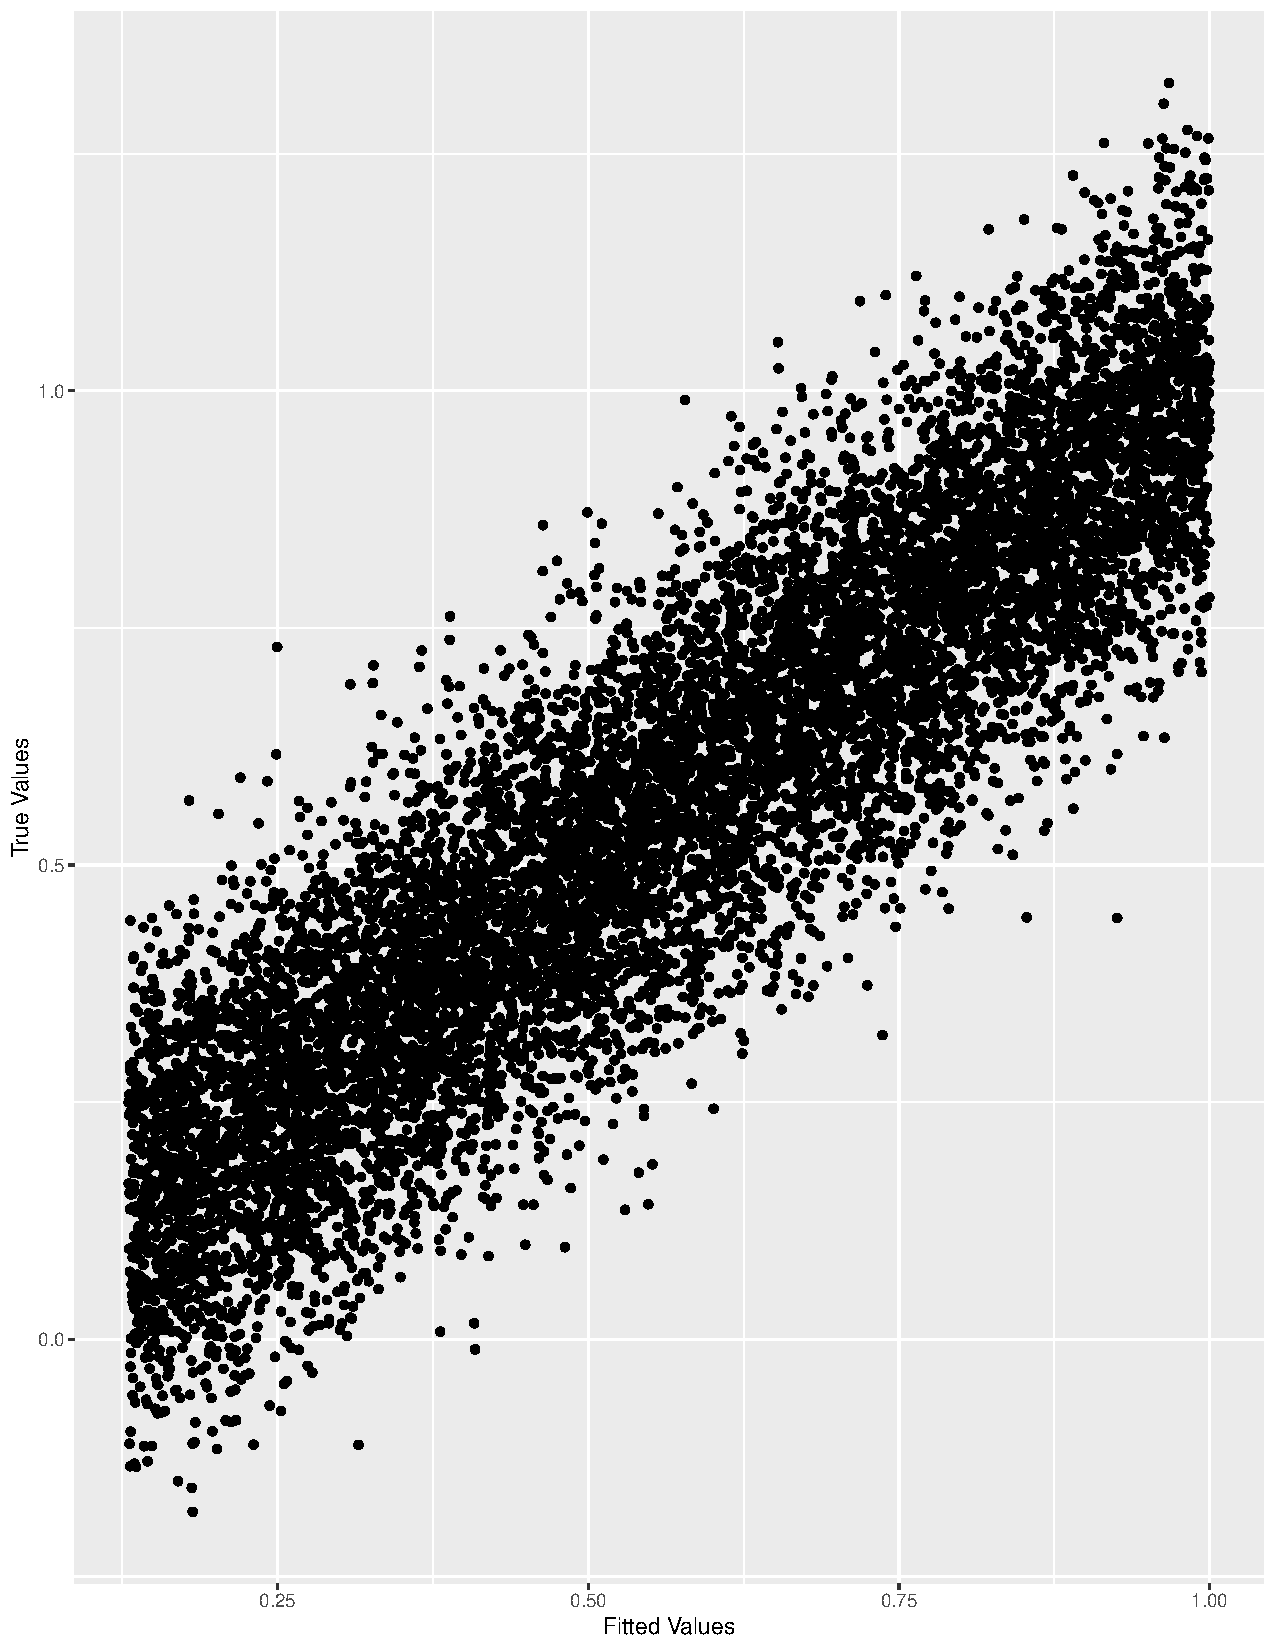
\includegraphics[width = 5cm]{plot/reg1}
\end{figure}
\end{frame}


\begin{frame}\frametitle{Introduction (5)}
Consider the following DGP:
\begin{itemize}
 \item 1,000 individuals over 10 periods. 
 \item $Y_{it} = \alpha_i + \beta X_{it} + \epsilon_{it}$
 \item Parametrization 
 \begin{itemize}
  \item $\beta = 1$
  \item $\alpha_i \sim uniform(-10,10)$
  \item $\epsilon_i \sim \N(0,1)$
 \end{itemize}
\end{itemize}
\end{frame}

\begin{frame}\frametitle{Pooled Estimation}
\begin{table}
\begin{center}
\begin{tabular}{l c }
\hline
 & Model 1 \\
\hline
(Intercept) & $-0.26^{*}$  \\
            & $(0.11)$     \\
c(xMat)     & $0.40^{***}$ \\
            & $(0.02)$     \\
\hline
R$^2$       & 0.04         \\
Adj. R$^2$  & 0.04         \\
Num. obs.   & 10000        \\
RMSE        & 5.73         \\
\hline
\multicolumn{2}{l}{\scriptsize{$^{***}p<0.001$, $^{**}p<0.01$, $^*p<0.05$}}
\end{tabular}
\caption{Statistical models}
\label{table:coefficients}
\end{center}
\end{table}
\end{frame}


\begin{frame}\frametitle{Fitted Values (2)}
\begin{figure}
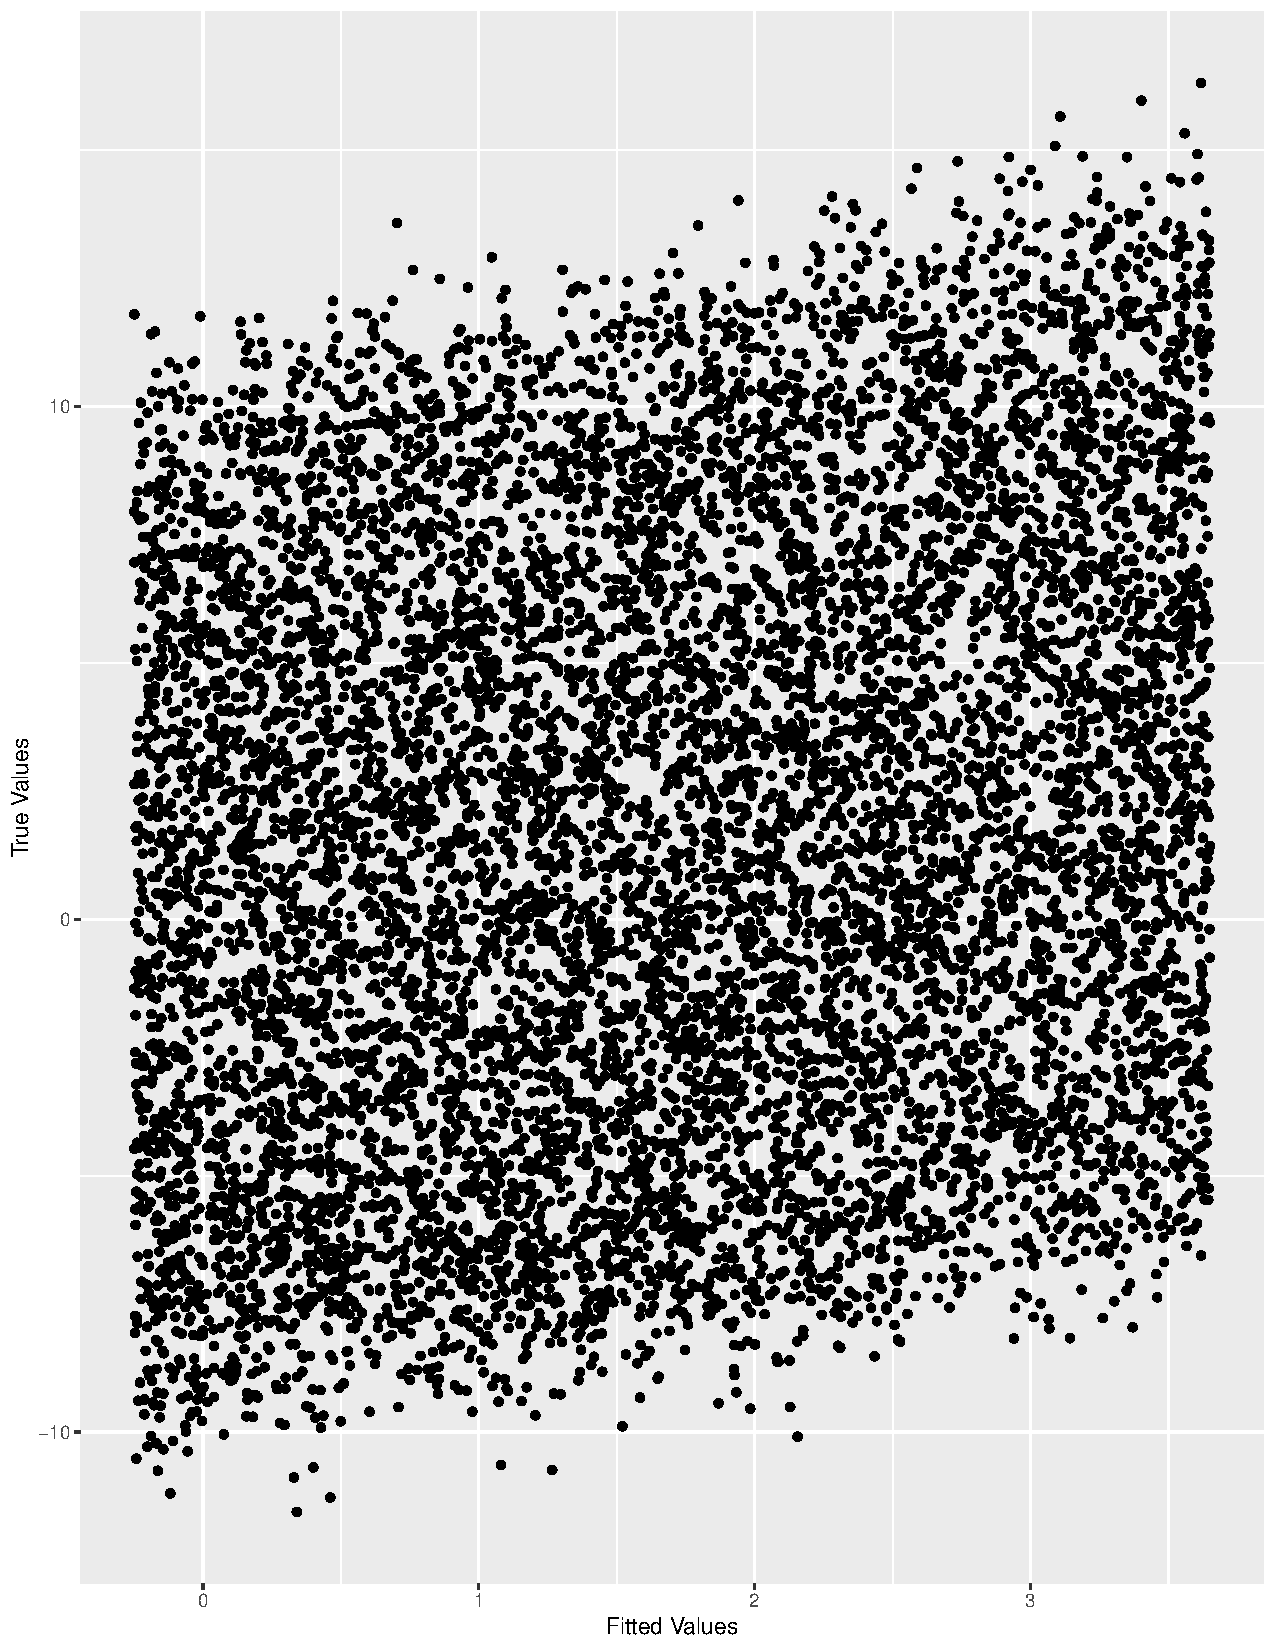
\includegraphics[width = 5cm]{plot/reg2}
\end{figure}
\end{frame}

\begin{frame}\frametitle{Effects}
\begin{itemize}
 \item Pooled Estimation is a good starting point.
 \item Individual VS Time Effect.
\end{itemize}
\end{frame}

\begin{frame}\frametitle{Individual Effects}
\begin{itemize}
 \item Fixed Effects
 \item Random Effects
 \item Examples: Return to Education
\end{itemize}
\end{frame}

\begin{frame}\frametitle{Time Effects}
\begin{itemize}
 \item Long Panel Case
 \item Example: Seasonality? 
\end{itemize}
\end{frame}

\begin{frame}\frametitle{Some Models (1)}
\begin{itemize}
 \item Pooled Estimator
 \begin{equation}
  Y_{it} = \alpha + \beta X_{it} + \epsilon_{it}
 \end{equation}
\item Problems
\end{itemize}
\end{frame}

\begin{frame}\frametitle{Some Models (2)}
\begin{itemize}
 \item Between Estimator
 \begin{equation}
  \bar{y}_i = \alpha_i + \beta \bar{x}_{i} + \bar{\epsilon}_{i}
 \end{equation}
\item Problems
\end{itemize}
\end{frame}

\begin{frame}\frametitle{Some Models (3)}
\begin{itemize}
 \item Within Estimator
 \begin{equation}
 y_{it} - \bar{y}_i =  \beta (x_{it} - \bar{x}_{i}) + 
 (\epsilon_{it} - \bar{\epsilon}_{i})
 \end{equation}
\item Problems
\end{itemize}
\end{frame}

\begin{frame}\frametitle{Some Models (4)}
\begin{itemize}
 \item First Difference Estimator
 \begin{equation}
 y_{it} - y_{i,t-1} =  \beta (x_{it} - x_{i,t-1}) + 
 (\epsilon_{it} - \epsilon_{i,t-1})
 \end{equation}
\item Problems
\end{itemize}

\end{frame}

\subsection{Applications}

\begin{frame}\frametitle{More Guns, Less Crime}
\begin{quote}
In a remarkable paper published in 1997, John Lott and David Mustard managed
to set the agenda for much subsequent work on the impact of guns on crime in America
by creating a massive data set of crime across all U.S. counties from 1977 through 1992
and amassing a powerful statistical argument that state laws enabling citizens to carry
concealed handguns had reduced crime.1
 The initial paper was followed a year later by
an even more comprehensive and sustained argument to the same effect in a book solely
authored by John Lott entitled More Guns, Less Crime (now in its second edition). 
\end{quote}
\end{frame}


\begin{frame}\frametitle{Data: Guns}
A data frame containing 1,173 observations on 13 variables.
\begin{itemize}
 \item state: factor indicating state.
\item year: factor indicating year.
\item violent: violent crime rate (incidents per 100,000 members of the population).
\item murder: murder rate (incidents per 100,000).
\item robbery: robbery rate (incidents per 100,000).
\item prisoners: incarceration rate in the state in the previous year 
\item afam: percent of state population that is African-American
\item cauc: percent of state population that is Caucasian, \item male: percent of state population that is male
\item population: state population, in millions of people.
\item income: real per capita personal income in the state (US \$).
\item density population per square mile of land area, divided by 1,000.
\item law factor. Does the state have a shall carry law in effect in that year?
\end{itemize}
\end{frame}

\begin{frame}\frametitle{Overtime Variation}
\begin{figure}
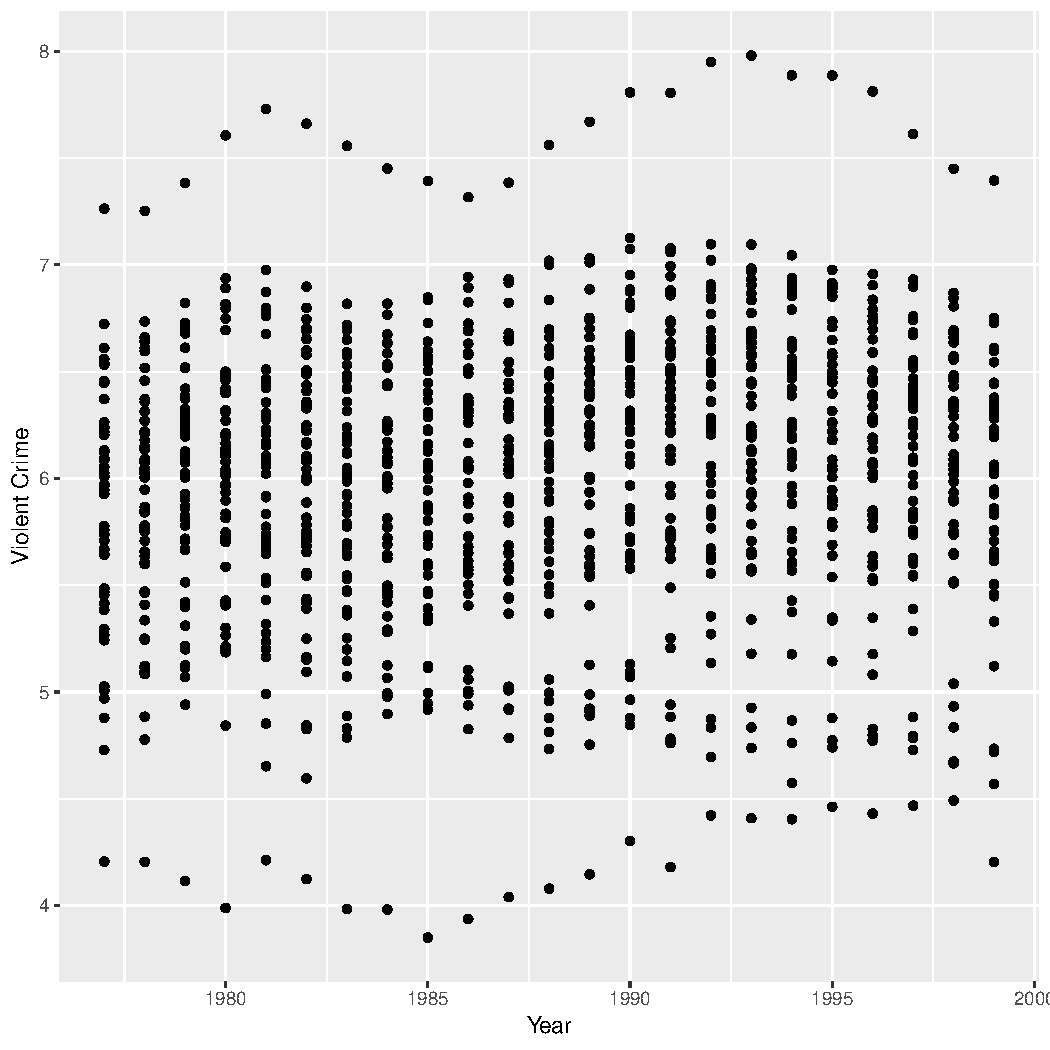
\includegraphics[width = 9cm]{plot/Time}
\end{figure}
\end{frame}


\begin{frame}\frametitle{Cross-sectional Variation (1)}
\begin{figure}
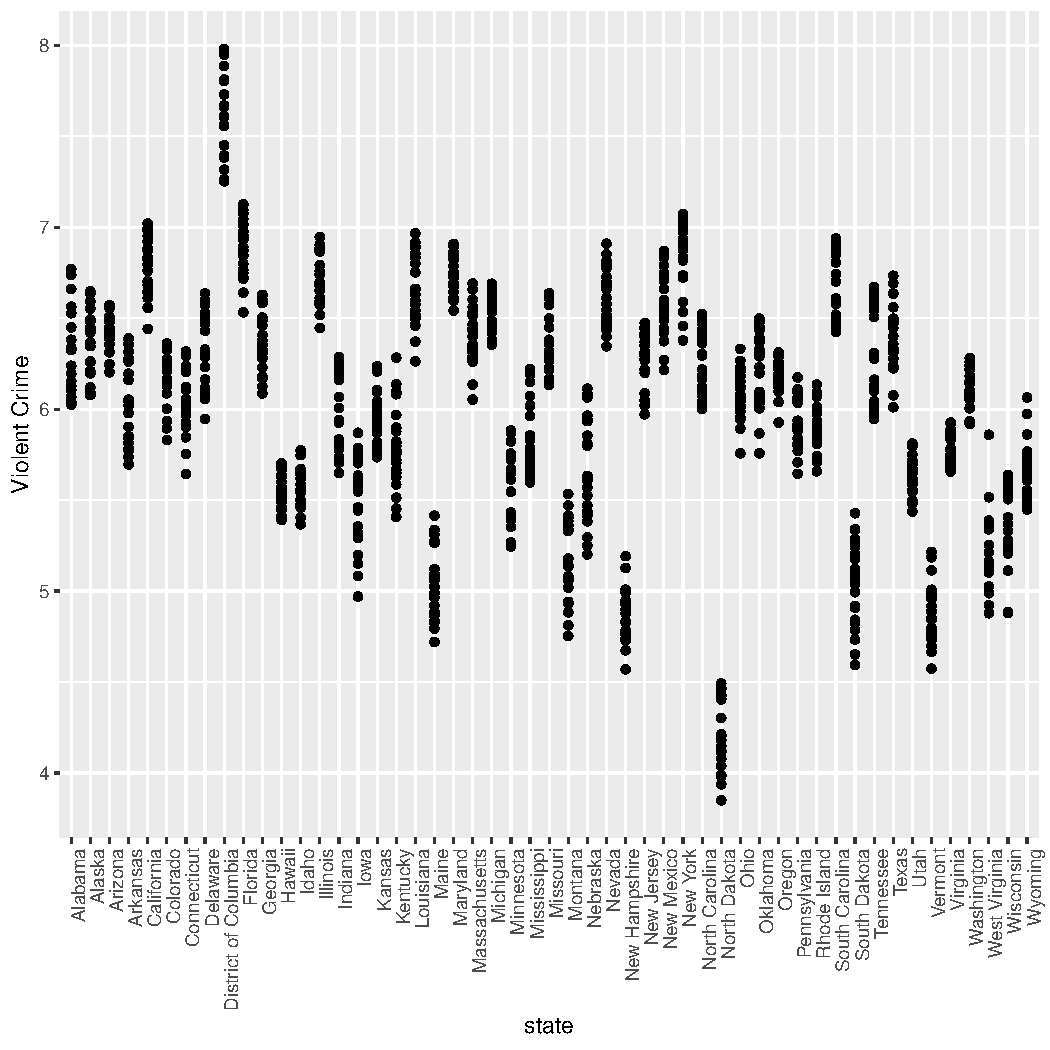
\includegraphics[width = 8cm]{plot/State}
\end{figure}
\end{frame}

\begin{frame}\frametitle{Cross-sectional Variation (2)}
\begin{figure}
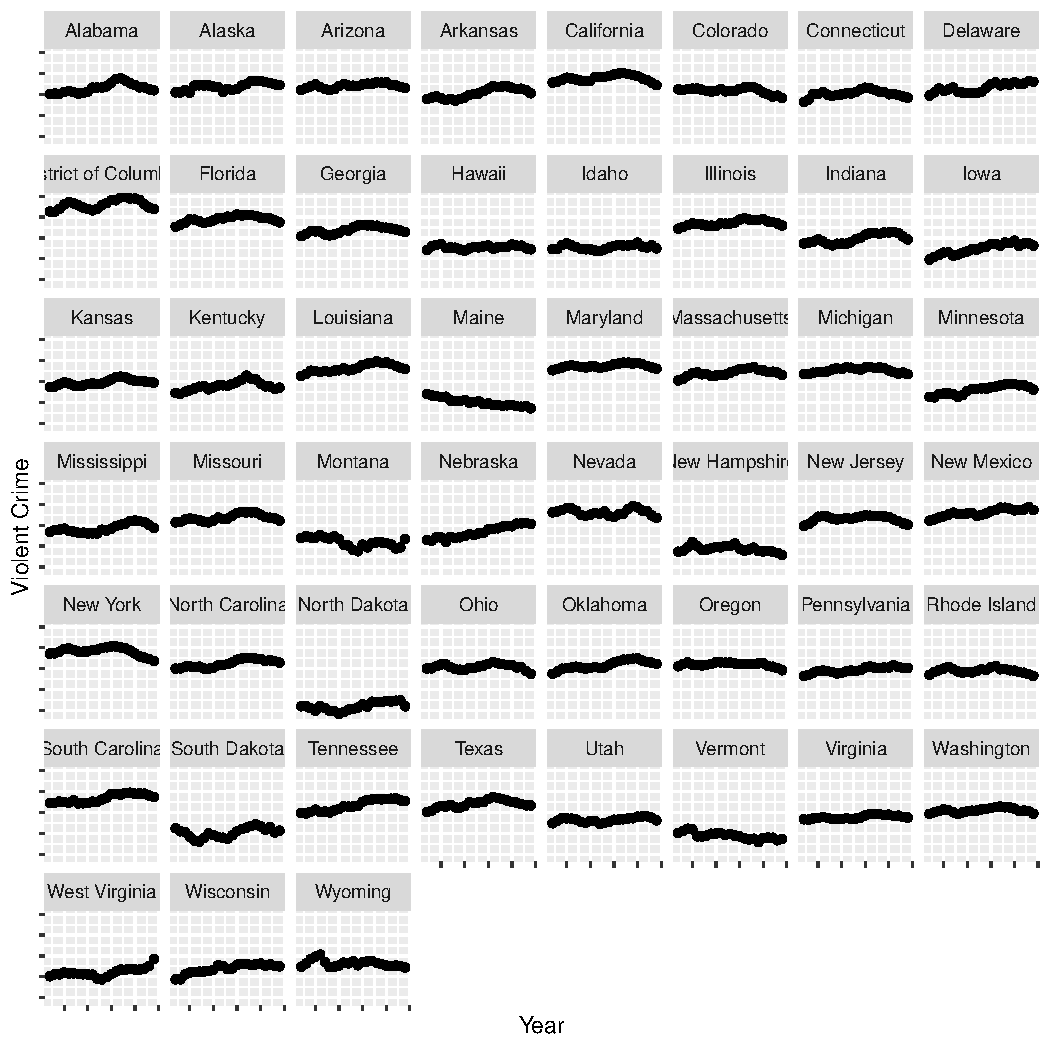
\includegraphics[width = 8cm]{plot/State_wrap}
\end{figure}
\end{frame}

\begin{frame}\frametitle{First regressions}
\begin{table}
\tiny
\begin{center}
\begin{tabular}{l c c c c }
\hline
  & \multicolumn{2}{c}{Violent Crime} & \multicolumn{2}{c}{Robbery}\\
 & Model 1 & Model 2 & Model 1 & Model 2 \\
\hline
(Intercept) & $6.13^{***}$  & $2.98^{***}$  & $4.87^{***}$  & $0.90$        \\
            & $(0.02)$      & $(0.54)$      & $(0.03)$      & $(0.77)$      \\
lawyes      & $-0.44^{***}$ & $-0.37^{***}$ & $-0.77^{***}$ & $-0.53^{***}$ \\
            & $(0.04)$      & $(0.03)$      & $(0.06)$      & $(0.05)$      \\
prisoners   &               & $0.00^{***}$  &               & $0.00^{***}$  \\
            &               & $(0.00)$      &               & $(0.00)$      \\
density     &               & $0.03^{*}$    &               & $0.09^{***}$  \\
            &               & $(0.01)$      &               & $(0.02)$      \\
income      &               & $0.00$        &               & $0.00^{***}$  \\
            &               & $(0.00)$      &               & $(0.00)$      \\
population  &               & $0.04^{***}$  &               & $0.08^{***}$  \\
            &               & $(0.00)$      &               & $(0.00)$      \\
afam        &               & $0.08^{***}$  &               & $0.10^{***}$  \\
            &               & $(0.02)$      &               & $(0.02)$      \\
cauc        &               & $0.03^{***}$  &               & $0.03^{*}$    \\
            &               & $(0.01)$      &               & $(0.01)$      \\
male        &               & $0.01$        &               & $0.03$        \\
            &               & $(0.01)$      &               & $(0.02)$      \\
\hline
R$^2$       & 0.09          & 0.56          & 0.12          & 0.60          \\
Adj. R$^2$  & 0.09          & 0.56          & 0.12          & 0.59          \\
Num. obs.   & 1173          & 1173          & 1173          & 1173          \\
RMSE        & 0.62          & 0.43          & 0.90          & 0.61          \\
\hline
\multicolumn{5}{l}{\scriptsize{$^{***}p<0.001$, $^{**}p<0.01$, $^*p<0.05$}}
\end{tabular}
\caption{Statistical models}
\label{table:coefficients}
\end{center}
\end{table}
\end{frame}

\begin{frame}\frametitle{Exploiting the Panel Structure}
\begin{table}
\tiny
\begin{center}
\begin{tabular}{l c c c }
\hline
 & Model 1 & Model 2 & Model 3 \\
\hline
(Intercept)               & $4.04^{***}$  & $3.09^{***}$  & $3.97^{***}$  \\
                          & $(0.39)$      & $(0.58)$      & $(0.47)$      \\
lawyes                    & $-0.05^{*}$   & $-0.29^{***}$ & $-0.03$       \\
                          & $(0.02)$      & $(0.03)$      & $(0.02)$      \\
prisoners                 & $-0.00$       & $0.00^{***}$  & $0.00$        \\
                          & $(0.00)$      & $(0.00)$      & $(0.00)$      \\
density                   & $-0.17^{*}$   & $-0.01$       & $-0.09$       \\
                          & $(0.09)$      & $(0.01)$      & $(0.08)$      \\
income                    & $-0.00$       & $0.00$        & $0.00$        \\
                          & $(0.00)$      & $(0.00)$      & $(0.00)$      \\
population                & $0.01$        & $0.04^{***}$  & $-0.00$       \\
                          & $(0.01)$      & $(0.00)$      & $(0.01)$      \\
afam                      & $0.10^{***}$  & $0.10^{***}$  & $0.03$        \\
                          & $(0.02)$      & $(0.02)$      & $(0.02)$      \\
cauc                      & $0.04^{***}$  & $0.04^{***}$  & $0.01$        \\
                          & $(0.01)$      & $(0.01)$      & $(0.01)$      \\
male                      & $-0.05^{***}$ & $-0.04^{*}$   & $0.07^{***}$  \\
                          & $(0.01)$      & $(0.02)$      & $(0.02)$      \\
State FE & YES & NO & YES \\
TIME FE & NO & YES & YES \\
\hline
R$^2$                     & 0.94          & 0.59          & 0.96          \\
Adj. R$^2$                & 0.94          & 0.58          & 0.95          \\
Num. obs.                 & 1173          & 1173          & 1173          \\
RMSE                      & 0.16          & 0.42          & 0.14          \\
\hline
\multicolumn{4}{l}{\scriptsize{$^{***}p<0.001$, $^{**}p<0.01$, $^*p<0.05$}}
\end{tabular}
\caption{Statistical models}
\label{table:coefficients}
\end{center}
\end{table}
\end{frame}


\begin{frame}\frametitle{Data: EmplUK}
Employment and Wages in the United Kingdom
\begin{itemize}
\item An unbalanced panel of 140 observations from 1976 to 1984
\item firm: firm index
\item year: year
\item sector: the sector of activity
\item emp: employment
\item wage: wages
\item capital: capital
\item output: output
\end{itemize}
\end{frame}

\begin{frame}\frametitle{Unbalanced Panel: Definitions}
\begin{itemize}
\item Unbalanced panel: Definition
\item What to do: Missing at random?
\end{itemize}
\end{frame}

\begin{frame}\frametitle{Unbalanced Panel: Solutions}
\begin{itemize}
\item Testing for missingness at random.
\item Missing at random
\begin{itemize}
\item Imputation
\item Full sample 
\item Non missing sample
\end{itemize}
\item Not missing at random
\begin{itemize}
\item Understand why?
\item Find an instrument
\end{itemize}
\end{itemize}
\end{frame}


\begin{frame}\frametitle{Description}
\begin{table}[!htbp] \centering 
\footnotesize
  \caption{} 
  \label{} 
\begin{tabular}{lccccccc} 
\\[-1.8ex]\hline 
\hline \\[-1.8ex] 
Statistic & \multicolumn{1}{c}{N} & \multicolumn{1}{c}{Mean} & \multicolumn{1}{c}{St. Dev.} & \multicolumn{1}{c}{Min} & \multicolumn{1}{c}{Pctl(25)} & \multicolumn{1}{c}{Pctl(75)} & \multicolumn{1}{c}{Max} \\ 
\hline \\[-1.8ex] 
firm & 1,031 & 73.204 & 41.233 & 1 & 37 & 110 & 140 \\ 
year & 1,031 & 1,979.651 & 2.216 & 1,976 & 1,978 & 1,981 & 1,984 \\ 
sector & 1,031 & 5.123 & 2.678 & 1 & 3 & 8 & 9 \\ 
emp & 1,031 & 7.892 & 15.935 & 0.104 & 1.180 & 7.020 & 108.562 \\ 
wage & 1,031 & 23.919 & 5.648 & 8.017 & 20.636 & 27.494 & 45.232 \\ 
capital & 1,031 & 2.507 & 6.249 & 0.012 & 0.221 & 1.501 & 47.108 \\ 
output & 1,031 & 103.801 & 9.938 & 86.900 & 97.098 & 110.603 & 128.365 \\ 
\hline \\[-1.8ex] 
\end{tabular} 
\end{table} 
\end{frame}

\begin{frame}\frametitle{Linear VS Log Specifications}
\begin{table}
\footnotesize
\begin{center}
\begin{tabular}{l c c }
\hline
 & Log & Linear \\
\hline
(Intercept)  & $0.34$        & $8.25^{**}$   \\
             & $(0.86)$      & $(3.11)$      \\
log(wage)    & $-0.37^{***}$ &               \\
             & $(0.06)$      &               \\
log(capital) & $0.81^{***}$  &               \\
             & $(0.01)$      &               \\
log(output)  & $0.48^{**}$   &               \\
             & $(0.18)$      &               \\
wage         &               & $-0.32^{***}$ \\
             &               & $(0.05)$      \\
capital      &               & $2.11^{***}$  \\
             &               & $(0.04)$      \\
output       &               & $0.02$        \\
             &               & $(0.03)$      \\
\hline
R$^2$        & 0.84          & 0.69          \\
Adj. R$^2$   & 0.84          & 0.69          \\
Num. obs.    & 1031          & 1031          \\
\hline
\multicolumn{3}{l}{\scriptsize{$^{***}p<0.001$, $^{**}p<0.01$, $^*p<0.05$}}
\end{tabular}
\caption{Statistical models}
\label{table:coefficients}
\end{center}
\end{table}
\end{frame}

\begin{frame}\frametitle{Fixed VS Random Effects}
\begin{table}
\footnotesize
\begin{center}
\begin{tabular}{l c c }
\hline
  & Random Effect & Fixed Effects \\
\hline
(Intercept)  & $2.20^{**}$   &       \\
             &  $(0.15)$     &       \\
log(wage)    & $-0.24^{***}$ &  $-0.61^{***}$             \\
             & $(0.05)$      &   $(0.03)$            \\
log(capital) & $0.61^{***}$  &  $0.56^{***}$            \\
             & $(0.07)$      &  $(0.02)$             \\
\hline
R$^2$        & 0.78          & 0.99          \\
Num. obs.    & 1031          & 1031          \\
\hline
\multicolumn{3}{l}{\scriptsize{$^{***}p<0.001$, $^{**}p<0.01$, $^*p<0.05$}}
\end{tabular}
\caption{Statistical models}
\label{table:coefficients}
\end{center}
\end{table}
\end{frame}

\begin{frame}\frametitle{Specification Problem}
\begin{itemize}
\item Choosing between random and fixed effects;
\item Durbin - Wu - Hausman Test 
\begin{equation}
H = (\beta_{FE} - \beta_{RE})' (Var(\beta_{FE}) - Var(\beta_{RE}))' (\beta_{FE} - \beta_{RE}) 
\end{equation}
\item $H \sim \chi_2(rank(Var(\beta_{FE}) - Var(\beta_{RE}))$
\end{itemize}
\end{frame}

\begin{frame}\frametitle{Data: US STATES PRODUCTION}
\begin{itemize}
\item state: state
\item year: year
\item region: the region
\item pcap: public capital stock
\item hwy: highway and streets
\item water: water and sewer facilities
\item util: other public buildings and structures
\item pc:private capital stock
\item gsp: gross state product
\item emp: labor input measured by the employment in nonagricultural payrolls
\item unemp: state unemployment rate
\end{itemize}
\end{frame}

\begin{frame}\frametitle{Specifications}
\begin{table}
\begin{center}
\begin{tabular}{l c c c }
\hline
 & Within & Between & First Difference \\
\hline
log(pcap)   & $-0.03$       & $0.18^{*}$   & $-0.01$       \\
            & $(0.03)$      & $(0.07)$     & $(0.05)$      \\
log(pc)     & $0.29^{***}$  & $0.30^{***}$ & $-0.03$       \\
            & $(0.03)$      & $(0.04)$     & $(0.02)$      \\
log(emp)    & $0.77^{***}$  & $0.58^{***}$ & $0.83^{***}$  \\
            & $(0.03)$      & $(0.06)$     & $(0.04)$      \\
unemp       & $-0.01^{***}$ & $-0.00$      & $-0.01^{***}$ \\
            & $(0.00)$      & $(0.01)$     & $(0.00)$      \\
(Intercept) &               & $1.59^{***}$ & $0.01^{***}$  \\
            &               & $(0.23)$     & $(0.00)$      \\
\hline
R$^2$       & 0.94          & 0.99         & 0.69          \\
Adj. R$^2$  & 0.94          & 0.99         & 0.69          \\
Num. obs.   & 816           & 48           & 768           \\
\hline
\multicolumn{4}{l}{\scriptsize{$^{***}p<0.001$, $^{**}p<0.01$, $^*p<0.05$}}
\end{tabular}
\caption{Statistical models}
\label{table:coefficients}
\end{center}
\end{table}
\end{frame}

\section{Econometrics of Policy Evaluation}

\begin{frame}
\tableofcontents[currentsection] 
\end{frame}

\begin{frame}\frametitle{Statement}
\begin{itemize}
\item Identify the causal effect of a policy
\begin{itemize}
 \item Minimum Wages on Employment
 \item Training on Wages
 \item Class size on Student Outcomes
 \item Welfare on Labor Supply
\end{itemize}
\item Essentially a self selection problem 
\end{itemize}

\end{frame}

\begin{frame}\frametitle{Evaluation Problem}
\begin{itemize}
\item Let $y_1$ denote the outcome with treatment 
 \item Let $y_0$ denote the outcome without treatment
 \item We are interested in the average treatment effect 
\begin{equation}
 ATE = E(y_1 - y_0)
\end{equation}
 \item Evaluation problem: An individual can not be in both states, we can not observe both $y_0$ and $y_1$.
 \item Another quantity is the average treatment effect of the treated (Let $w$ be an indicator of treatment).
 \begin{equation}
  ATT = E(y_1 - y_0 \mid w=1)
 \end{equation}
\end{itemize}
\end{frame}

\begin{frame}\frametitle{Assumptions}
Under which assumptions can you do a DiD?
\begin{itemize}
 \item Stable Unit Treatment Value
Assumption (SUTVA):  potential outcomes for each person i
 are unrelated to the treatment status of other individuals
\item  Random Assignment.
 The treatment assignment is random i.e we have an independent, identically distributed
sample from the population
\end{itemize}
\end{frame}

\begin{frame}\frametitle{Threat to Validity}
\begin{itemize}
 \item Pre-trend
 \item Placebo Effect
 \item Rubin Effect
\end{itemize}
\end{frame}

\begin{frame}\frametitle{DiD as a Linear Regression}
Consider 
\begin{equation}
 Y_{it} = \alpha + \delta Post_t + \gamma D_i + \beta Post_t D_i + \epsilon_{it}
\end{equation}
Where
\begin{itemize}
 \item $D_i=1$ if treated, 0 otherwise
 \item $Post_t=1$ after the implementation of the policy 
\end{itemize}
\end{frame}

\begin{frame}\frametitle{Alternative Method: Regression discontinuity}
The Key intuition for RDD is that we have an understanding of the mechanism which underlies the assignment of treatment. Specifically, assignment to treatment depends on a single variable. In the sharp, regression discontinuity design, the running variable fully determines the treatment

\begin{equation}
D_i = \begin{cases} 1, & \mbox{If } X_i > X_0 \\ 0, & \mbox{If } X_i < X_0 \end{cases}
\end{equation}
\end{frame}

\begin{frame}\frametitle{Idea}
\begin{figure}
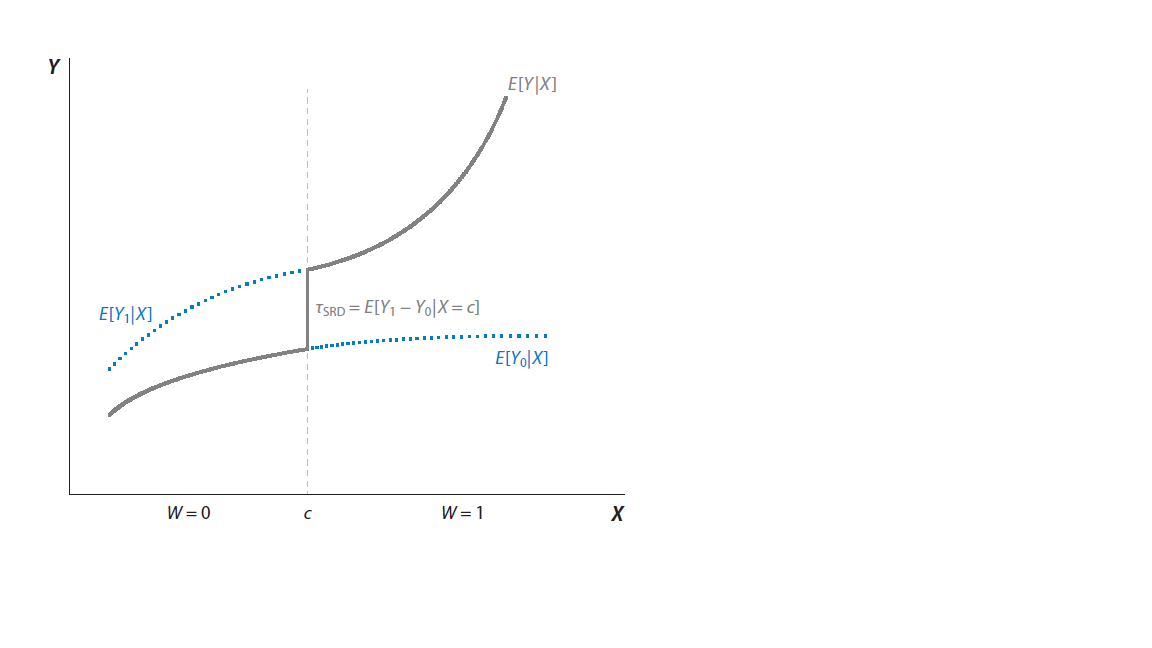
\includegraphics[width = 10cm]{plot/Idea}
\end{figure}
\end{frame}


\begin{frame}\frametitle{Some examples (1)}
\begin{figure}
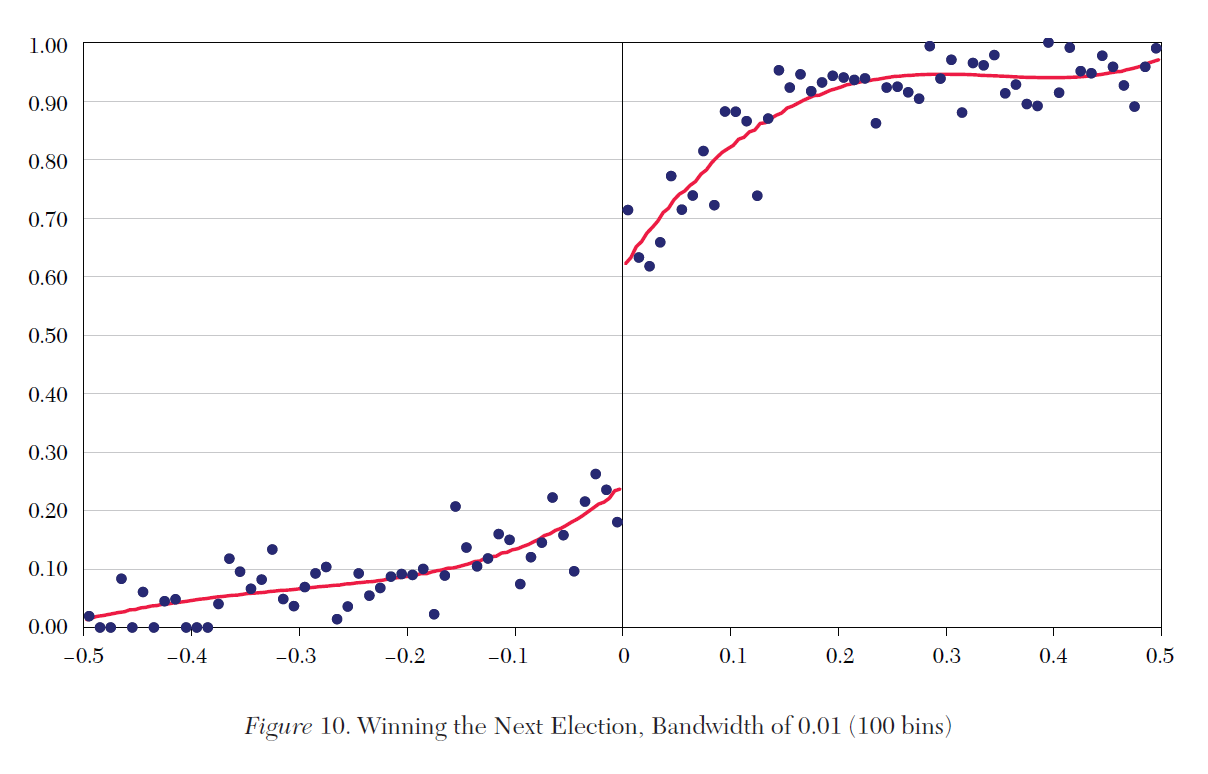
\includegraphics[width = 10cm]{plot/ProbWinning}
\end{figure}
\end{frame}

\begin{frame}\frametitle{Some examples (2)}
\begin{figure}
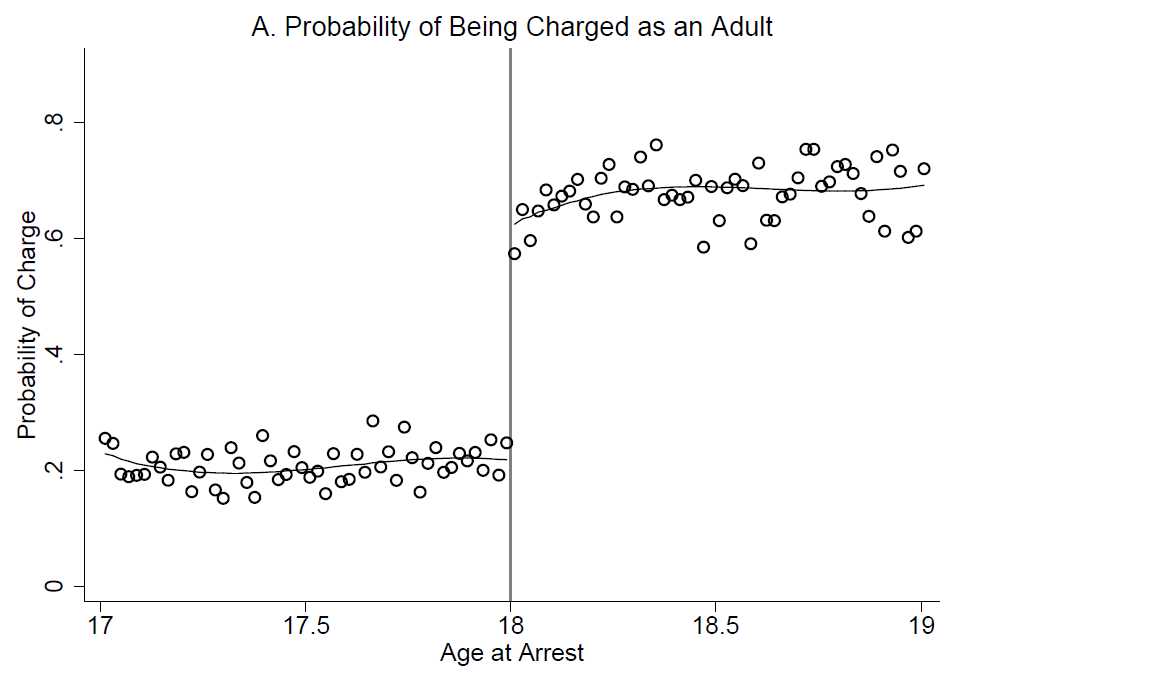
\includegraphics[width = 10cm]{plot/Charged}
\end{figure}
\end{frame}

\begin{frame}\frametitle{Some examples (3)}
\begin{figure}
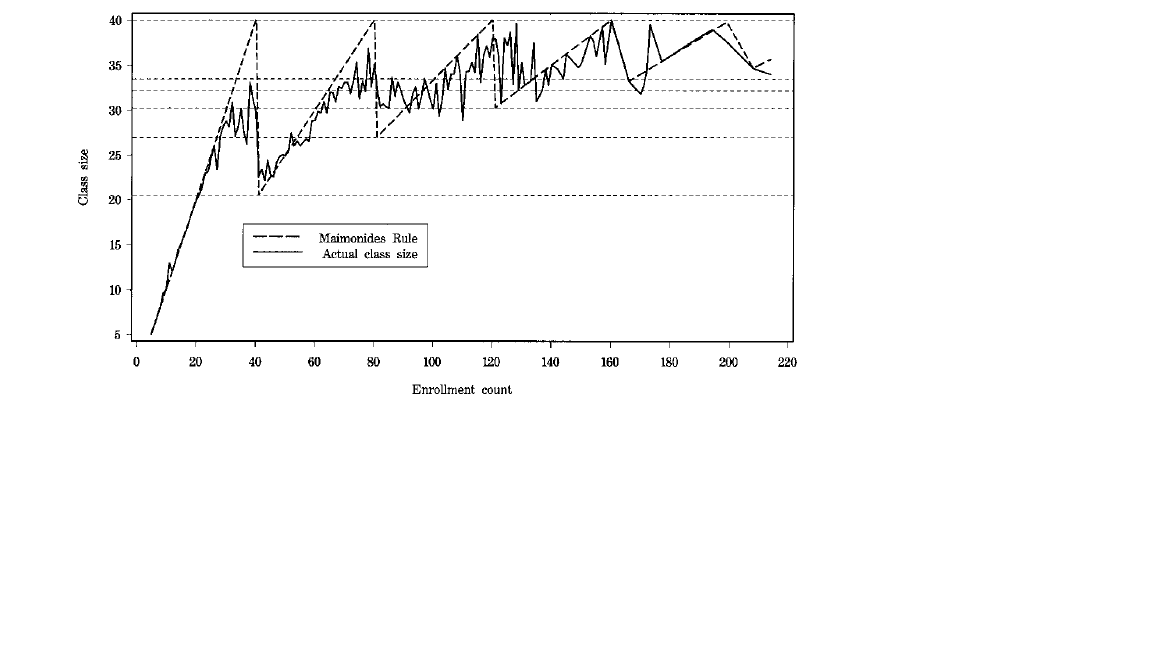
\includegraphics[width = 10cm]{plot/MaimonidesRule}
\end{figure}
\end{frame}

\begin{frame}\frametitle{Explanation (1)}
\begin{quote}
Twenty five children may be put in charge of one
teacher. If the number in the class exceeds
twenty five but is not more than forty, he should
have an assistant to help with the instruction. If
there are more than forty, two teachers must be
appointed. 
\end{quote}
\end{frame}

\begin{frame}\frametitle{Explanation (2)}
\begin{itemize}
\item A law prevents class size to exceed say 30
\item If cohorts are of average size 90 but fluctuates
\item If cohort size is 91-96, we end up four classrooms of size 22 to 24, while if cohort size is 85-90, we end up with three classrooms of size 28 to 30. 
\end{itemize}
Angrist and Lavy (1999): Comparing test outcomes between students who are randomly assigned to the small vs large classes gives you a credible estimate of the effect of class size on academic performance. 10\% decrease in class size increases test score by about 0.2 to 0.3 standard deviations. 
\end{frame}

\section{Applications}

\begin{frame}\frametitle{Uses and Abuses of Empirical Evidence in the Death Penalty Debate}
\begin{itemize}
 \item Deterrance Effect of the death penalty
 \item What can we say?
\end{itemize}
\end{frame}

\begin{frame}\frametitle{Evidence and Abuse (1)}
\begin{figure}
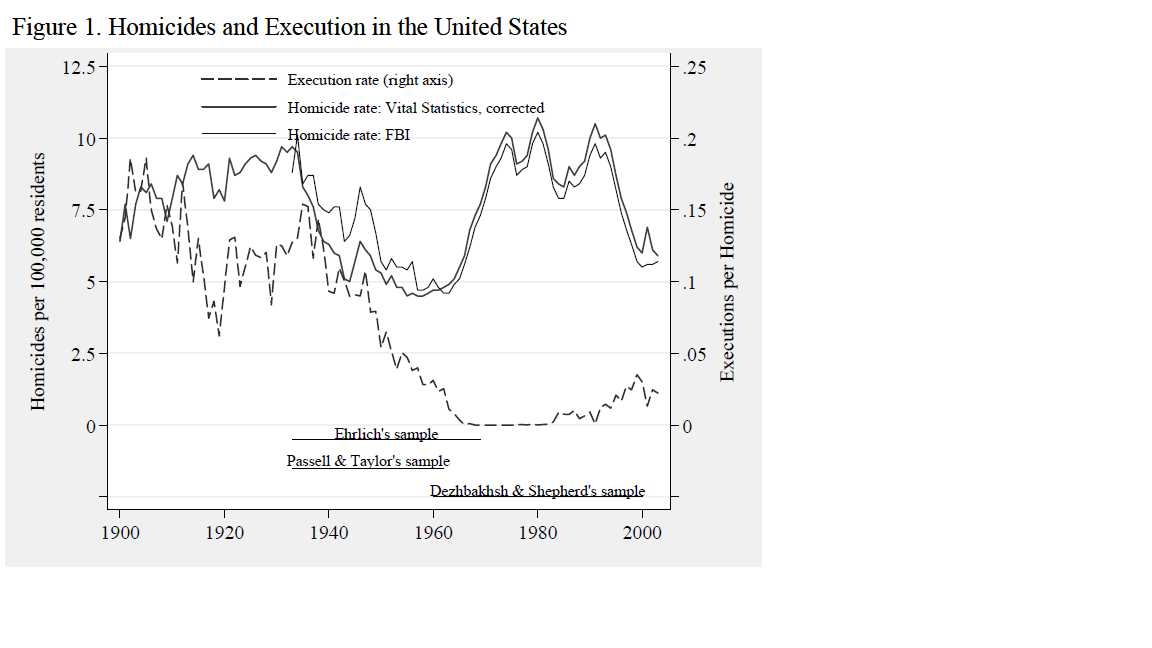
\includegraphics[width = 10cm]{plot/HomicidesExecution}
\end{figure}
\end{frame}

\begin{frame}\frametitle{Evidence and Abuse (2)}
\begin{figure}
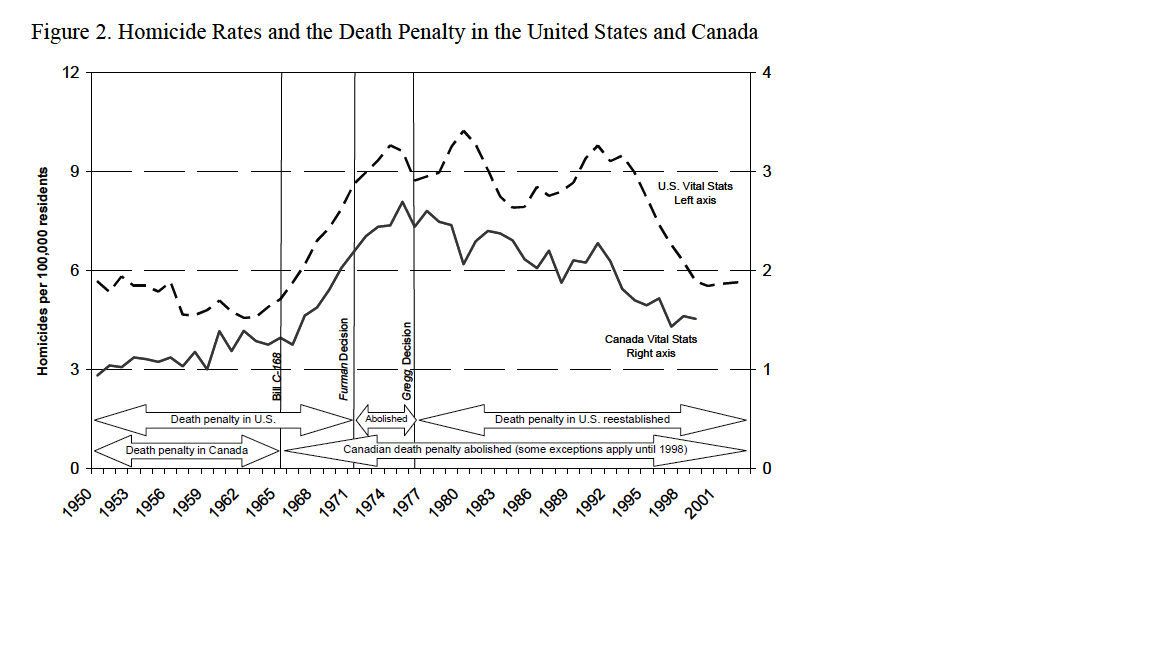
\includegraphics[width = 10cm]{plot/USCanada}
\end{figure}
\end{frame}

\begin{frame}\frametitle{Evidence and Abuse (3)}
\begin{figure}
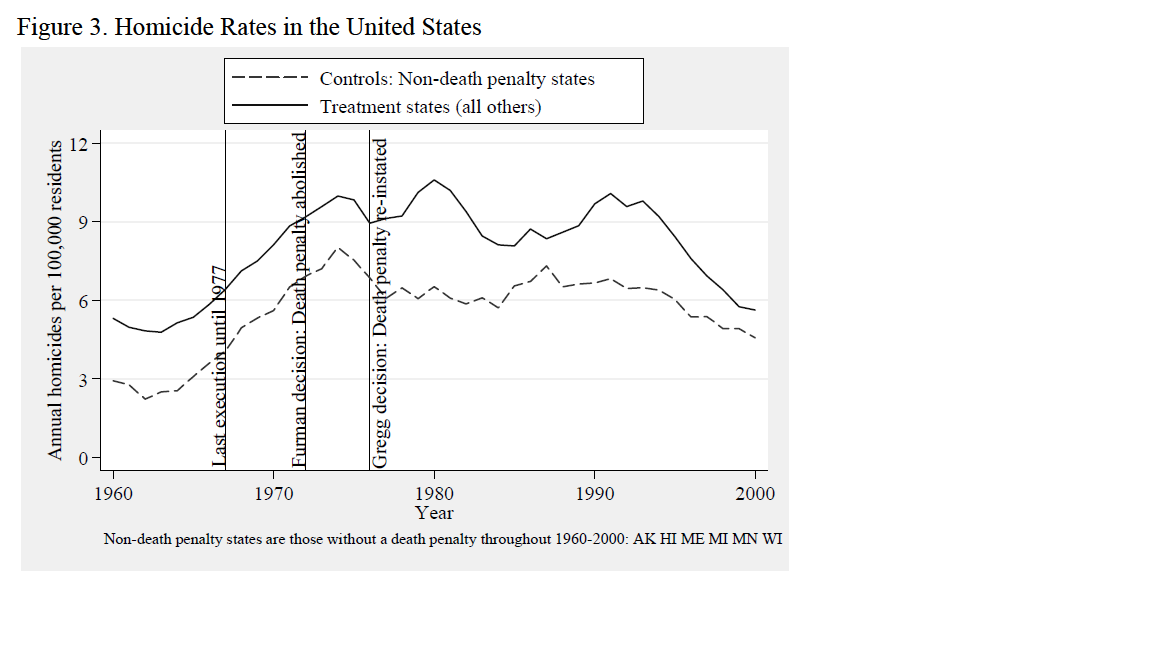
\includegraphics[width = 10cm]{plot/Nondeath}
\end{figure}
\end{frame}

\begin{frame}\frametitle{Evidence and Abuse (4)}
\begin{figure}
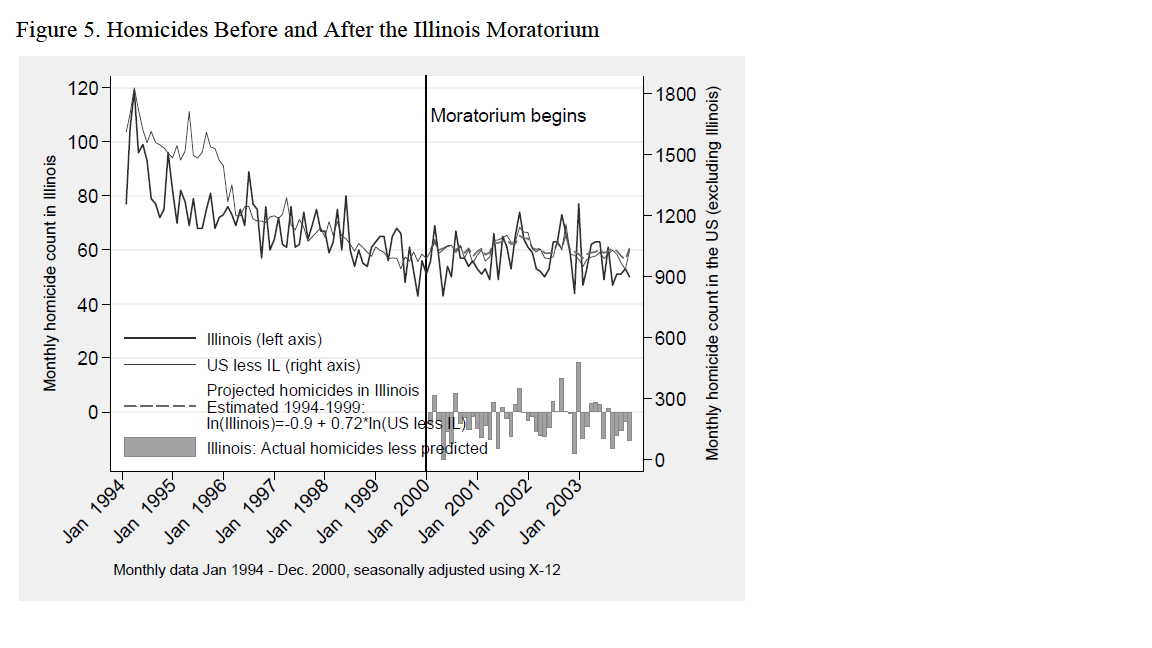
\includegraphics[width = 10cm]{plot/Illinois}
\end{figure}
\end{frame}

\begin{frame}\frametitle{Evidence and Abuse (5)}
\begin{figure}
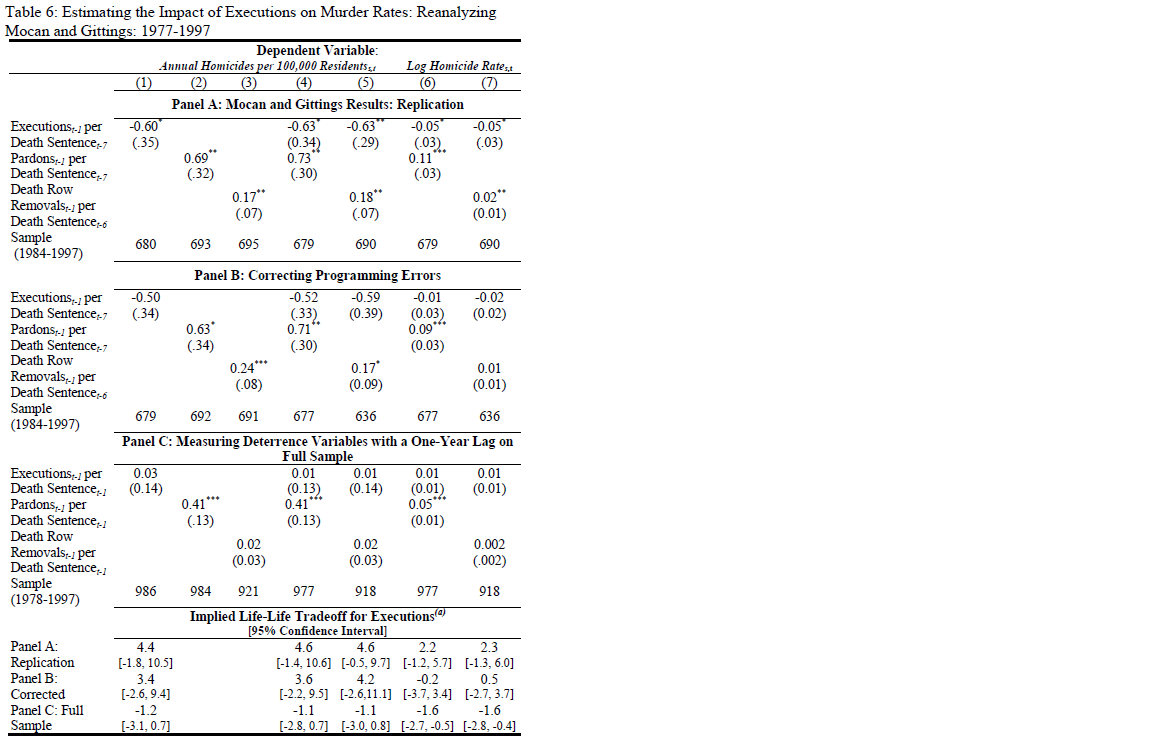
\includegraphics[width = 10cm]{plot/Table}
\end{figure}
\end{frame}

\section{Recap Issues day}

\begin{frame}
\tableofcontents[currentsection] 
\end{frame}

\begin{frame}\frametitle{Summary}
\begin{itemize}
\item Immigration
\item Intergenerational Mobility
\item Minimum Wages
\end{itemize}
\end{frame}

\begin{frame}\frametitle{Issues}
\begin{itemize}
\item Causal Inference is hard!
\item Problems
\begin{itemize}
\item Data selection
\item Specification
\end{itemize}
\end{itemize}
\end{frame}


\section{Discrete Choice with Panel Data}

\begin{frame}
\tableofcontents[currentsection] 
\end{frame}

\begin{frame}\frametitle{Motivation}
\begin{itemize}
\item Determinant of an outcome variable which varies over time.
\item Example
\begin{itemize}
\item Fertility 
\item Retirement
\item Binary decisions with life-cycle component
\item \ldots
\end{itemize}
\end{itemize}
\end{frame}

\begin{frame}\frametitle{Probit and Logit}
\begin{itemize}
\item Consider an individual specific effect, such that 
\begin{equation}
Pr(y_{it}=1) = F(x_{it} \beta + \alpha_i)
\end{equation}
\item Likelihood can be written naturally
\end{itemize}
\end{frame}

\begin{frame}\frametitle{Fixed effect estimation}
\begin{itemize}
\item Probit case - kind of complicated - incidental parameter problem. 
\item Logit case - conditional MLE
\item No quasi-differencing estimator
\end{itemize}
\end{frame}

\begin{frame}\frametitle{Random effect }
\begin{itemize}
\item Probit - complicated numerically - requires numerical integration
\item Logit - relatively simple
\end{itemize}
\end{frame}

\section{Survival Analysis}

\begin{frame}
\tableofcontents[currentsection] 
\end{frame}

\begin{frame}\frametitle{Transition Data}
\begin{itemize}
 \item Panel Data
 \item Outcome variable is a duration: length of time until an event occurs (or a spell ends)
 \item Examples
 \begin{itemize}
  \item Unemployment
  \item Strike 
  \item Time to (buy a house, marry, divorce....)
 \end{itemize}
\end{itemize}
\end{frame}

\begin{frame}\frametitle{Basic concepts}
\begin{itemize}
\item Density: $f(t)$
\item Distribution: $F(t)$ 
\item Survival Function: $S(t)=1-F(t)$
\item Hazard rate: $\lambda(t) = \lim_{h \rightarrow 0} \dfrac{Pr[t<T<t+h \mid T\geq t]}{h} = \dfrac{f(t)}{1-F(t)} = \dfrac{f(t)}{S(t)}$
\end{itemize}
\end{frame}

\begin{frame}\frametitle{Estimation methods}
\begin{itemize}
\item Nonparametric: Kaplan Meier
\item Parametric: Exponential, Weibull,
\item Semi-parametric: Cox Proportional Hazard
\end{itemize}
\end{frame}

\begin{frame}\frametitle{Likelihood based Estimation}
\begin{itemize}
\item Censoring
\begin{equation}
d_i = \begin{cases} 1, & \mbox{no censoring} \\ 0, & \mbox{right censoring } \end{cases}
\end{equation}
\item Likelihood
\begin{equation}
\log \Lik(\theta) = d_i \log f(t_i \mid X,\theta) + (1-d_i) \log S(t_i \mid X,\theta)
\end{equation}
\end{itemize}
\end{frame}

\section{Final words}

\begin{frame}
\tableofcontents[currentsection] 
\end{frame}


\begin{frame}\frametitle{Student Evaluations}
\begin{itemize}
\item Coding - 60 \% (due April 16th)
\item Reading notes - 40\% (due April 19th)
\end{itemize}
\end{frame}


\begin{frame}\frametitle{Course Evaluation}
\url{https://duke.qualtrics.com/jfe/form/SV_9t7Bige533zblMp}
\end{frame}

\end{document}


